
\chapter{Estado del arte}
\label{cha:estadoarte}

En este capítulo se expondrán en detalle los conceptos más relevantes relacionados con el proyecto, además de las  herramientas y el software empleado para el desarrollo del mismo. El fin principal de este apartado es entrar en el marco teórico que engloba al proyecto para una mayor compresión de su diseño en los siguientes capítulos.

\section{Smart grids}
%[http://www.smartgrids.eu]
Una smart grid o red energética inteligente se puede definir como aquella red que es capaz de suministrar electricidad de forma eficiente a sus usuarios según la información que adquiere de los mismos. Es decir, se plantea un esquema energético distribuido basado en una comunicación bidireccional entre la compañía eléctrica y los clientes. A partir de este modelo, el sistema registrará las acciones de cada uno de los usuarios conectados y diferenciará entre aquellos que se comportan como consumidores, los que son generadores de energía o los prosumidores, que desarrollan ambos papeles.



%[https://www.redalyc.org/articulo.oa?id=411534385004]
%[Díaz, C. & Hernández, J. (2011). Smart Grid: Las TICs y la modernización de las redes de energía eléctrica- Estado del Arte. Revista S&T, 9(18), 53-81.]
\begin{figure}[h!]
    \centering
    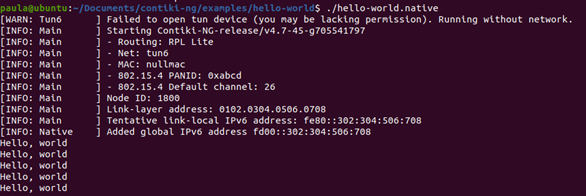
\includegraphics[width=0.8\textwidth]{contiki hello world}
    %\includegraphics[]{smart grids 1}
    \caption{Ejecución en modo nativo}
    \label{fig:smart grids 1}
\end{figure}


%%%
se plantea un modelo de red eléctrica 
basado en tres pilares: generación distribuida, autonomía en su control y 
tecnologías de la información para transmitir y manejar todos los datos.
En este sentido ha surgido la nueva generación de redes eléctricas inteligentes 
o smart grids, las cuales han sido objeto de numerosos estudios de desarrollo e 
implantación.



Las smart grids o redes eléctricas inteligentes son una forma de gestión eficiente 
de la electricidad. A pesar de que no existe una definición universal 
estandarizada, la Plataforma Tecnológica Europea de smart grids (smart grids: 
European Technology Platform, http://www.smartgrids.eu )


Se puede resumir el fin que persiguen las smart grids en lo siguiente:
 Garantizar óptimos niveles de fiabilidad, seguridad y calidad del 
suministro.
 Reducir el impacto medioambiental del sistema eléctrico de suministro.
 Proporcionar a los consumidores mayor información de oferta.
 Permitir a los consumidores formar una parte importante en la 
optimización del sistema.
 Facilitar y mejorar la conexión y el funcionamiento de los generadores de 
todo tipo de tamaños y tecnologías.


\section{Redes LLN/encaminamiento eficiente}







\section{IoTorii}



\section{Contiki-ng}
Contiki se trata de un sistema operativo ligero para el tratamiento de redes de sensores o dispositivos IoT de baja capacidad. El proyecto fue creado en 2002 por Adam Dunkels, Bjorn Gronvall y Thiemo Voigt, ingenieros del Swedish Institute of Computer Science. 
% [https://ieeexplore.ieee.org/document/1367266]

Es un software de código abierto y gracias a esto y a la colaboración de otras empresas, con el tiempo ha podido ir evolucionando y actualizándose. Se puede acceder a su última versión desde su repositorio de GitHub. [https://github.com/contiki-ng/contiki-ng]

Contiki tiene como núcleo un kernel y su programación se basa en el tratamiento de los eventos de los diferentes procesos implicados para ofrecer una ejecución multithreading con requisa. Es un sistema operativo portable, soporta la concurrencia y es eficiente en el uso de memoria, ya que todos los hilos comparten una misma pila.
%[http://eprints.ugd.edu.mk/16096/ ///// http://www.tfzr.rs/itro/Zbornik%20ITRO%202016.pdf]


\subsection{Simulador Cooja}
En redes IoT a gran escala la existencia de multitud de dispositivos dificultan el desarrollo y la depuración de los procesos de cada uno de los nodos. Para simplificar el funcionamiento de Contiki se ofrece como opción la aplicación Cooja.

Cooja es un simulador gráfico basado en Java que permite monitorizar redes IoT de cualquier tamaño o topología. Para ello, se debe definir un número determinado de nodos o motas y el tipo de plataforma en la que se va a simular el comportamiento del programa. Se dispone de varios paquetes que proveen diferentes tipos de dispositivos hardware para emular. Así, se permite probar el código antes de ejecutarlo en un controlador hardware real.

Además, Cooja permite guardar la información y los resultados de las simulaciones realizadas en una estructura XML mediante ficheros de extensión *.csc.

%%%////Para ejecutar Cooja se debe acceder al directorio tools/cooja y ejecutar el comando ant
%https://github.com/contiki-ng/contiki-ng/wiki/Tutorial:-Running-Contiki%E2%80%90NG-in-Cooja

\subsection{Ejemplos}
Para tener un primer contacto con el software de Contiki se recomienda probar su funcionamiento con algunos de los ejemplos de proyectos que este incluye en el directorio examples/.

\subsubsection{Hello World}
% [https://github.com/contiki-ng/contiki-ng/wiki/Tutorial:-Hello,-World!]
El programa en cuestión comenzará un proceso que imprimirá por consola el mensaje Hello, World cada diez segundos. A continuación, se muestran las ejecuciones en modo nativo o por defecto y en Cooja.

En el modo nativo se ejecutará el programa directamente desde el terminal. Para compilar en este modo se necesita el comando make hello-world.native TARGET=native. En la figura \ref{fig:contiki hello world} se puede observar la secuencia de mensajes obtenida.


\begin{figure}[h!]
    \centering
    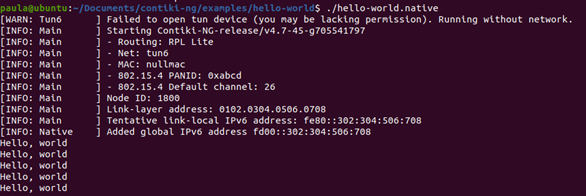
\includegraphics[width=0.8\textwidth]{contiki hello world}
    %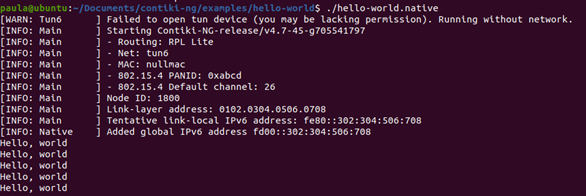
\includegraphics[]{contiki hello world}
    \caption{Ejecución en modo nativo}
    \label{fig:contiki hello world}
\end{figure}

Por otra parte, con el uso del simulador gráfico Cooja, la compilación se podrá realizar a través del propio simulador o mediante el comando make hello-world.cooja TARGET=cooja. En este caso, se se han definido dos motas que intercambiarán los mensajes entre sí como se muestra en la ventana de salida.


\begin{figure}[h!]
    \centering
    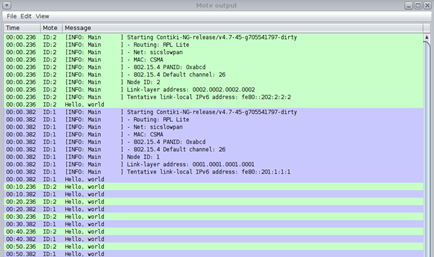
\includegraphics[width=0.8\textwidth]{contiki hello world 3}
    \caption{Ejecución en modo nativo}
    \label{fig:contiki hello world 3}
\end{figure}







\section{Brite}
%[https://open.bu.edu/handle/2144/3752?show=full]
%[https://github.com/NETSERV-UAH/BRITE]
Brite (Boston University Representative Internet Topology Generator) se presenta como una herramienta de apoyo para la creación de topologías de red aleatorias. 

El software fue desarrollado por miembros del Departamento de Ciencias Computacionales de la Universidad de Boston con el fin de establecer un algoritmo flexible que soporte la generación de diversos modelos de topologías. La configuración de cada uno de los modelos se basa principalmente en los parámetros de entrada que se definen. Estos especificarán propiedades de la red como la posición de los nodos, las características del ancho de banda de los enlaces o el número de conexiones de cada uno de los nodos.


\section{Mininet}











